\begin{frame}
    \frametitle{Material}
    
    Vídeos para armar estas slides:
    \begin{itemize}
        \item Cyrill Stachniss Bayes: \url{https://youtu.be/0lKHFJpaZvE}
        \item Cyrill Stachniss KF y EKF: \url{https://youtu.be/E-6paM_Iwfc}
        \item Chebrolu EKF Localization: \url{https://youtu.be/PiCC-SxWlH8}
        \item Cyrill Stachniss Particle Filter: \url{https://youtu.be/MsYlueVDLI0}
        \item Slides de ECI 2012
        \item Seminario de curso: CS373 Udacity Programming a Robotic Car
    \end{itemize}
    
\end{frame}

\begin{frame}
    \frametitle{Temario para estas slides}
    
    \begin{itemize}
        \item Bayes filter
        \item kalman filter
        \item Particle filter
    \end{itemize}
    
    
\end{frame}

\begin{frame}{Localización}
	\begin{block}{Localización}
		Es la habilidad que posee una máquina para localizarse en el espacio.
	\end{block}
\end{frame}


\begin{frame}
	\frametitle{Estimación de estado}
	
	\note{Información obtenida de Cyrill Stachniss Bayes: https://youtu.be/0lKHFJpaZvE}
	
	\begin{itemize}
		\item  Estimar el estado $\state$ de un systema dada las observaciones $\observation$ y comandos de control $\controlCommand$
		\item Objetivo:
	\end{itemize}
	
	\begin{equation}
		p\left(\state_{t} | \observation_{1:t}, \controlCommand_{1:t} \right)
	\end{equation}
	
	Estimación de estado recursiva: Se trata de estimar $\state_{t}$ el estado actual utilizando también el estado inmediatamente anterior $\state_{t-1}$.
\end{frame}

\begin{frame}{Filtro de Bayes Recursivo}
    \begin{block}{Ejemplo}
        \begin{itemize}
            
            \item Dado un robot en un mundo de una dimensión, sin conocimiento de en donde se encuentra
            \item El robot se puede mover hacia delante o atrás
            \item Supongamos además que hay tres puertas (\alert{landmarks}), el robot puede detectar si se encuentra al lado de una puerta o no.
        \end{itemize}
    \end{block}
\end{frame}

\begin{frame}{Filtro de Bayes Recursivo: Posición inicial}
    Como en un principio el robot desconoce cual es su posición entonces es igualmente posible que se encuentre en cualquier punto del mundo (\alert{belief}). Esto lo podemos representar matemáticamente diciendo que la \alert{función de distribución de probabilidad} del robot es \alert{uniforme} sobre el mundo en que se encuentra.
    \begin{center}
        \includegraphics<1>[height=2cm]{./images/monte_carlo_uniform.pdf}
    \end{center}
    
\end{frame}

\begin{frame}{Filtro de Bayes Recursivo: Medición}
    
    Si el robot sensa que se encuentra al lado de una puerta entonces la creencia de su ubicación se se ve alterada de la siguiente manera:
    
    \begin{center}
        \includegraphics<1>[height=2cm]{./images/monte_carlo_sensing.pdf}
    \end{center}
    
    
    Esta nueva función representa otra distribución de probabilidades llamada \alert{Posterior belief}.
    
    La función Posterior belief es la mejor representación de la posición del robot actualmente. Cada ``loma'' representa la evaluación de su posición con respecto a una puerta.
    
\end{frame}

\begin{frame}{Filtro de Bayes Recursivo: Movimiento}
    
    Si el robot se mueve hacia la derecha la creencia es cambiada de acuerdo al movimiento.
    Así mismo como el movimiento del robot es inexacto, al trasladarse su incertidumbre crece, dicho de otra manera, las lomas son aplanadas. Este aplanamiento matemáticamente se lleva a cabo por medio de la operación de \alert{convolución} entre la función Posterior belief y la función que describe la distancia recorrida.
    
    \begin{center}
        \includegraphics<1>[height=2cm]{./images/monte_carlo_moving.pdf}
    \end{center}
    
    La operación de convolución mide la superposición mientras se desliza una funcion sobre otra.
    
\end{frame}

\begin{frame}{Filtro de Bayes Recursivo: Segunda medición}
    Supongamos que el robot luego de haberse movido sensa nuevamente que se encuentre al lado de una puerta entonces, como antes, la probabilidad se incrementara por un cierto factor la función de probabilidad donde haya una puerta.
    
    \begin{center}
        \includegraphics<1>[height=2cm]{./images/monte_carlo_sensing2.pdf}
    \end{center}
\end{frame}

\begin{frame}{Filtro de Bayes Recursivo: Segundo movimiento}
	Supongamos que el robot se mueve nuevamente...
	
	\begin{center}
		\includegraphics<1>[height=2cm]{./images/monte_carlo_moving2.pdf}
	\end{center}
\end{frame}


\begin{frame}
	\frametitle{Estimación de estado}
	
	\note{Información obtenida de Cyrill Stachniss Bayes: https://youtu.be/0lKHFJpaZvE}
	
	\begin{itemize}
		\item  Estimar el estado $\state$ de un systema dada las observaciones $\observation$ y comandos de control $\controlCommand$
		\item Objetivo:
	\end{itemize}
	
	\begin{equation}
		p\left(\state_{t} | \observation_{1:t}, \controlCommand_{1:t} \right)
	\end{equation}
	
	Estimación de estado recursiva: Se trata de estimar $\state_{t}$ el estado actual utilizando también el estado inmediatamente anterior $\state_{t-1}$.
\end{frame}


\begin{frame}
	\frametitle{Estimación de estado}
	
	\note{Información obtenida de Cyrill Stachniss Bayes: https://youtu.be/0lKHFJpaZvE}
	Estamos interesados en la creencia (\emph{belief}) del sistema de dónde está en el tiempo $t$:
    
    \begin{columns}[t]
        \begin{column}{0.5\textwidth}
        	\begin{equation}
            bel(\state_{t}) = p\left(\state_{t} | \observation_{1:t}, \controlCommand_{1:t} \right)
            \end{equation}
        \end{column}
        \begin{column}{0.5\textwidth}
        (ecuación de estimación de estado o definición de distribución de probabilidad)
        \end{column}
    \end{columns}
    \vspace{1cm}
    La ecuación se puede leer dónde estoy ahora $\state_{t}$ dada todas las observaciones $\observation_{1:t}$ y todos los comandos de control $\controlCommand_{1:t}$

    Ahora vamos a simplificar la distribución utilizando la Regla de Bayes:

\end{frame}


\begin{frame}
    \frametitle{Derivación del Filtro de Bayes Recursivo}
    
    \note{Información obtenida de Cyrill Stachniss Bayes: https://youtu.be/0lKHFJpaZvE}
    \begin{align*}
        \only<1->{
            bel(\state_{t}) &= p\left(\state_{t} | \observation_{1:t}, \controlCommand_{1:t} \right)\\
        }
        \only<2->{
                            &= \eta \, p\left(\observation_{t} |\state_{t}, \observation_{1:t-1}, \controlCommand_{1:t} \right) p\left(\state_{t} | \observation_{1:t-1}, \controlCommand_{1:t} \right) \quad \text{donde $\eta$ es una constante de normalización}\\
            }
        \only<3->{
                            &= \eta \, p\left(\observation_{t} |\state_{t} \right) p\left(\state_{t} | \observation_{1:t-1}, \controlCommand_{1:t} \right)\\
                }
        \only<4->{
                            &= \eta \, p\left(\observation_{t} |\state_{t} \right) \int p\left(\state_{t} | \state_{t-1}, \observation_{1:t-1}, \controlCommand_{1:t} \right) p\left(\state_{t-1} | \observation_{1:t-1}, \controlCommand_{1:t} \right) d \state_{t-1}\\
                }
        \only<5->{
                            &= \eta \, p\left(\observation_{t} |\state_{t} \right) \int p\left(\state_{t} | \state_{t-1}, \controlCommand_{t} \right) p\left(\state_{t-1} | \observation_{1:t-1}, \controlCommand_{1:t} \right) d \state_{t-1}\\
                }
        \only<6->{
                            &= \eta \, p\left(\observation_{t} |\state_{t} \right) \int p\left(\state_{t} | \state_{t-1}, \controlCommand_{t} \right) p\left(\state_{t-1} | \observation_{1:t-1}, \alert{\controlCommand_{1:t-1}} \right) d \state_{t-1}\\
                }
        \only<7->{
                            &= \eta \, p\left(\observation_{t} |\state_{t} \right) \int p\left(\state_{t} | \state_{t-1}, \controlCommand_{t} \right) \alert{bel(\state_{t-1})} d \state_{t-1}
                }
    \end{align*}
    \only<2>{Regla de Bayes}
    \only<3>{Markov assumption. Lo que mido ahora solo depende del estado anterior y es independiente de las mediciones y los comandos anteriores.}
    \only<4>{Ley de probabilidad total. Es decir, integramos sobre todos los estados anteriores posibles.}
    \only<5>{Markov assumption.}
    \only<6>{Independence assumption.} \note{Perdemos información ya que ayumismos independencia. Asumismo que un comando futuro no nos ayuda en saber nuestra pose actual. Esto no siempre es cierto.}
    \only<7>{Término recursivo!}
    \note{Luego se pueden seguir haciendo asumciones, por ejemplo asumir que las probabilidades son gaussianas. Lo cual no es cierto en general.}
\end{frame}

\begin{frame}{Paso de Predicción y Paso de Corrección}
    \note{Información obtenida de Cyrill Stachniss Bayes: https://youtu.be/0lKHFJpaZvE}
    \begin{itemize}
        \item El Filtro de Bayes puede ser escrito como un proceso de dos pasos
        \begin{equation*}
        bel(\state_{t}) = \eta \, p\left(\observation_{t} |\state_{t} \right) \int p\left(\state_{t} | \state_{t-1}, \controlCommand_{t} \right) bel(\state_{t-1}) d \state_{t-1}
        \end{equation*}
        \item Paso de Predicción
        \begin{equation*}
            \overline{bel}(\state_{t}) = \int p\left(\state_{t} | \state_{t-1}, \controlCommand_{t} \right) bel(\state_{t-1}) d \state_{t-1}
        \end{equation*}
        \item Paso de Corrección
        \begin{equation*}
            bel(\state_{t}) = \eta \, p\left(\observation_{t} |\state_{t} \right) \overline{bel}(\state_{t})
        \end{equation*}
    \end{itemize}

    \note{El paso de predicción: predice dónde vamos a estar dado los comandos de control}
    \note{El paso de corrección: teniendo en cuenta las mediciones actuales corrije la pose predicha}
    
\end{frame}

\begin{frame}{Motion model y observation model}
    \note{Información obtenida de Cyrill Stachniss Bayes: https://youtu.be/0lKHFJpaZvE}
    \begin{itemize}
         \item Paso de Predicción
        \begin{equation*}
            \overline{bel}(\state_{t}) = \int \underbrace{p\left(\state_{t} | \state_{t-1}, \controlCommand_{t} \right)}_{\text{Motion model}} bel(\state_{t-1}) d \state_{t-1}
        \end{equation*}
        \item Paso de Corrección
        \begin{equation*}
            bel(\state_{t}) = \eta \underbrace{p\left(\observation_{t} |\state_{t} \right)}_{\text{\makebox[0pt]{Observation model (Measurement model o Sensor model)}}} \overline{bel}(\state_{t})
        \end{equation*}
    \end{itemize}
    
    \note{El paso de predicción: predice dónde vamos a estar dado los comandos de control}
    \note{El paso de corrección: teniendo en cuenta las mediciones actuales corrije la pose predicha}
    
\end{frame}

\begin{frame}{Diferentes implementaciones}
    \note{Información obtenida de Cyrill Stachniss Bayes: https://youtu.be/0lKHFJpaZvE}
    \begin{itemize}
        \item El Filtro de Bayes es un {\bf framework} estimación de estado recursiva
        \item Hay diferentes implementaciones
        \item Diferentes Propiedades:
        \begin{itemize}
            \item Modelos lineales vs no-lineales para el modelo de movimiento y observación
            \item Utilización de distribuciones de probabilidad solamente Gausianas? 
            \item Filtros paramétricos y no-paramétricos (representar la distribución de probabilidad de manera paramétrica o no-paramétrica)
            \item ...
        \end{itemize}
    \end{itemize}
    
\end{frame}

\begin{frame}{Filtros populares}
    \note{Información obtenida de Cyrill Stachniss Bayes: https://youtu.be/0lKHFJpaZvE}
    \begin{itemize}
        \item Kalman Filter
        \begin{itemize}
            \item Utiliza distribuciones de probabilidad Gaussianas
            \item Solo funciona con modelo de movimiento y observación lineales
        \end{itemize}
        \item Extended Kalman Filter (EKF)
        \begin{itemize}
            \item Utiliza distribuciones de probabilidad Gaussianas
            \item {\bf Lineariza} los modelos de movimiento y observación no lineales por medio de aproximación de Taylor
        \end{itemize}
        \item Particle filter
        \begin{itemize}
            \item No-paramétrico 
            \item Modelos de distribuciones probabilísticas arbitrarias, es decir no todo es Gaussiano (etapa de sampleo de muestras)
        \end{itemize}
    \end{itemize}

    \note{- Nonparametric filters represent posterior state as a function of previous state.
    - Nonparametric filters does not rely on a fixed functional form of
    posterior.
    - Histogram filter and Particle filter represent state space and posterior as a finite set of data.
    - There is usually a trade-off between efficiency and level of detail of data.}
    \note{el precio a pagar es que tiene un costo computacional muy alto}
\end{frame}

\begin{frame}{Motion Model}
    \note{Información obtenida de Cyrill Stachniss Bayes: https://youtu.be/0lKHFJpaZvE}
    \begin{equation*}
        \overline{bel}(\state_{t}) = \int \underbrace{p\left(\state_{t} | \state_{t-1}, \controlCommand_{t} \right)}_{\text{Motion model}} bel(\state_{t-1}) d \state_{t-1}
    \end{equation*}
\end{frame}

\begin{frame}{Ejemplo: Movimiento basado en odometría}
	\note{Información obtenida de Cyrill Stachniss Bayes: https://youtu.be/0lKHFJpaZvE}
	
	\begin{figure}[!h]
		\centering
		\subfloat[]
		{
			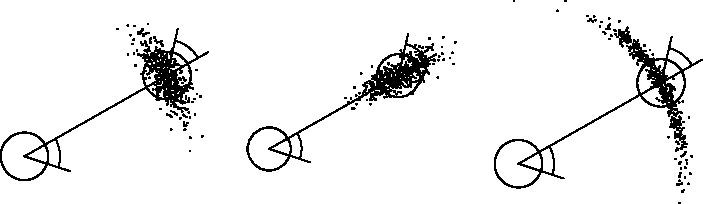
\includegraphics[width=0.6\columnwidth]{./images/samping_odometry_motion_model.pdf}
		}\\
		\subfloat[Muestras del motion model]
		{
			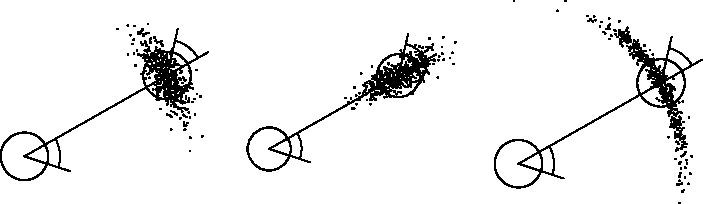
\includegraphics[width=0.6\columnwidth]{./images/samping_odometry_motion_model.pdf}
		}
	\end{figure}
	
	
\end{frame}

\begin{frame}{Observation model}
    \note{Información obtenida de Cyrill Stachniss Bayes: https://youtu.be/0lKHFJpaZvE}
    \begin{equation*}
        bel(\state_{t}) = \eta \underbrace{p\left(\observation_{t} |\state_{t} \right)}_{\text{\makebox[0pt]{Observation model (Measurement model o Sensor model)}}} \overline{bel}(\state_{t})
    \end{equation*}
\end{frame}

\begin{frame}{Ejemplo: Movimiento basado en odometría}
    \note{Información obtenida de Cyrill Stachniss Bayes: https://youtu.be/0lKHFJpaZvE}
    
   	\begin{figure}[!h]
    	\centering
    	\subfloat[]
    	{
    		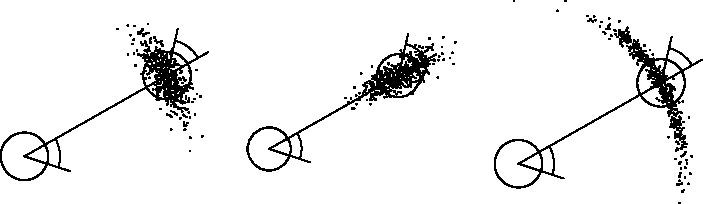
\includegraphics[width=0.6\columnwidth]{./images/samping_odometry_motion_model.pdf}
    	}\\
    	\subfloat[Muestras del motion model]
    	{
    		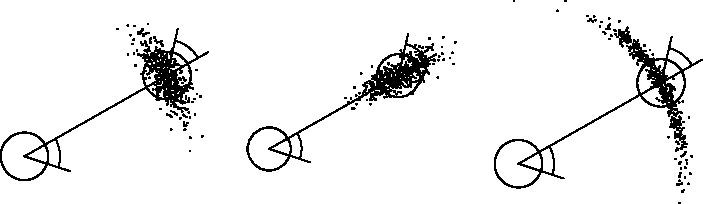
\includegraphics[width=0.6\columnwidth]{./images/samping_odometry_motion_model.pdf}
    	}
    \end{figure}


\end{frame}

\begin{frame}
	\frametitle{Extended Kalman Filter}
	
	\note{Información obtenida de:
		Cyrill Stachniss KF y EKF: https://youtu.be/E-6paM_Iwfc
		Chebrolu EKF Localization: https://youtu.be/PiCC-SxWlH8}
    
    https://automaticaddison.com/extended-kalman-filter-ekf-with-python-code-example/
    https://github.com/shangzhouye/EKF-SLAM-on-Turtlebot3
    
    https://github.com/ser94mor/sensor-fusion
    
    https://github.com/AtsushiSakai/PythonRobotics
    
    Puede ser que el tp sea en python no mas y el tp final hacerlo en ROS2.
    
    https://github.com/debbynirwan/mcl
    
    
\end{frame}

